\documentclass[11pt]{article}

\usepackage[T1]{fontenc}
\usepackage[utf8]{inputenc}
\usepackage{lmodern}
\usepackage{microtype}
\usepackage[a4paper,margin=2.15cm]{geometry}
\usepackage{amsmath,amssymb,bm}
\usepackage{booktabs}
\usepackage{float}
\usepackage{graphicx}
\usepackage{siunitx}
\usepackage{authblk}
\usepackage{enumitem}
\usepackage{xcolor}
\usepackage{xurl}
\usepackage{hyperref}
\usepackage[nameinlink,capitalise]{cleveref}
\usepackage[backend=biber,style=numeric,sorting=none,maxbibnames=99]{biblatex}
\addbibresource{references.bib}

\hypersetup{
  colorlinks=true,
  linkcolor=blue!45!black,
  citecolor=blue!45!black,
  urlcolor=blue!55!black,
  pdftitle={Hardware-Oriented Hidden-Code-Sampling-Inspired Certification on a 60-Qubit Superconducting Processor},
  pdfauthor={Abdelmalik Berrada}
}
\sisetup{group-separator={,},group-minimum-digits=4}
\setlist[itemize]{leftmargin=1.25em,itemsep=2pt,topsep=3pt}
\setlist[enumerate]{leftmargin=1.6em,itemsep=4pt,topsep=4pt}
\emergencystretch=2em

\title{\textbf{Hardware-Oriented Hidden-Code-Sampling-Inspired Certification\\on a 60-Qubit Superconducting Processor}}
\author{Abdelmalik Berrada}
\affil{Independent Researcher, Casablanca, Morocco}
\date{31 July 2026}

\begin{document}
\maketitle

\begin{abstract}
We report a hardware-oriented quantum sampling experiment motivated by Hidden Code Sampling (HCS), while explicitly not claiming an end-to-end implementation of the original HCS \textsc{PeakVerification}--\textsc{SyndromeVerification} protocol. A full-width 60-qubit circuit derived from a sparse trivariate-bicycle CSS construction was embedded without swaps on a 108-qubit superconducting processor and compiled to native $R_X$, $R_Z$, and controlled-$Z$ operations. The base circuit contains 180 logical two-qubit rotations and 360 native controlled-$Z$ gates; local unitary folding produced stress instances with factors 1, 3, and 5 and respectively 360, 1080, and 1800 controlled-$Z$ gates.

A pilot run was used only to identify and freeze an endian-corrected two-feature local parity witness. The final certificate used confirmatory QPU executions submitted after the freeze, with fresh pre- and post-experiment assignment calibrations. Each science circuit received \num{10000} shots, and each of four calibration patterns received \num{4000} shots in both calibration periods. We construct simultaneous finite-shot lower confidence bounds by combining Clopper--Pearson calibration intervals, a pre/post drift hull, inverse assignment-channel correction, an empirical Bernstein bound, and worst-case optimization over the calibration box. The certified margins above a registered adversarial baseline plus generalization penalty are 0.2953, 0.2858, and 0.3148 at folds 1, 3, and 5, respectively. All three folds pass; the maximum calibration-parameter drift is 0.0065.

Within a preregistered classical attack suite, the best recorded simulation proxy is $9.70\times10^{7}$ operations, versus 27 witness-verification operations, yielding a conditional gap $\gamma=\log_{10}(C_{\mathrm{classical}}/C_{\mathrm{verify}})=6.555$. This is an operation-count certificate relative to registered attacks, not a wall-clock quantum advantage claim and not a full-distribution total-variation certificate. The public source package includes sanitized QASM, aggregate certificate data, and verification metadata; the immutable private audit chain is retained separately.
\end{abstract}

\noindent\textbf{Scope statement.}
The experiment is HCS-inspired: it uses code-derived structure, peaked local observables, and a verification/simulation cost comparison. It does not implement the complete logical/syndrome HCS output test and therefore does not claim an experimental realization of the exact HCS protocol.

\section{Introduction}
Quantum sampling experiments face a verification bottleneck: the most direct validation methods often require classical simulation of the same computation whose intractability is being tested. Hidden Code Sampling (HCS) was proposed to address this tension by using quantum-error-correcting-code structure to create conditionally peaked distributions with efficient verification procedures~\cite{deshpande2025hcs}. Related directions include verifiable IQP schemes~\cite{bremner2025stabilizer}, code--hardware co-design for hard IQP sampling~\cite{hangleiter2024hypercube}, experimentally verifiable measurement-based random sampling~\cite{ringbauer2024randomsampling}, and hardware demonstrations of heuristic peaked circuits~\cite{gharibyan2025peaked}. The latter also illustrates the necessity of aggressive classical red-teaming: a later structure-specific contraction method substantially reduced the reported classical cost~\cite{kremer2026peaked}.

This work studies a deliberately narrower question: can a code-derived, topology-matched, full-width circuit support a reproducible positive local-witness certificate on current hardware, under fresh calibration, finite-shot uncertainty, independent confirmation, and registered classical attacks? The answer is positive for one frozen 60-qubit instance. The experiment is designed as a hardware-oriented bridge toward HCS rather than as a substitute for the complete HCS verification protocol.

The main contributions are:
\begin{enumerate}
  \item a sparse $[[60,4,\geq3]]$ CSS-derived circuit construction embedded on a live 108-qubit superconducting topology with no swap insertion;
  \item a strict pilot/confirmation split in which pilot counts are excluded from the final certificate and all scientific choices are frozen before confirmatory submission;
  \item a calibration-robust simultaneous finite-shot certificate evaluated at local unitary-fold stress levels 1, 3, and 5;
  \item a machine-verifiable provenance chain using frozen manifests, QASM hashes, disjoint pilot/confirmatory identities, and authorization-hash validation; and
  \item a conditional verification/simulation operation-count gap against a preregistered suite of tensor-network, MPS, Schr\"odinger--Feynman, stabilizer-decomposition, and statevector proxies.
\end{enumerate}

\section{Relation to Hidden Code Sampling and Prior Work}
The original HCS proposal samples from a code-structured quantum process and verifies both a peaked logical component and the syndrome distribution~\cite{deshpande2025hcs}. The present experiment retains three HCS-motivated ingredients: structured CSS codes, local peaked observables, and a large disparity between the cost of checking a witness and the registered cost of simulating the circuit. It changes the experimental verification target from the full logical/syndrome distribution to a frozen local parity witness. Consequently, the result should be read as an HCS-inspired hardware experiment.

The closest experimental comparison is heuristic peaked-circuit sampling on Quantinuum hardware~\cite{gharibyan2025peaked}; those circuits use a different construction and were later exposed to a structure-specific classical simulation~\cite{kremer2026peaked}. Verifiable random sampling has also been demonstrated in measurement-based computation using stabilizer checks~\cite{ringbauer2024randomsampling}. In the code-co-design direction, hypercube IQP circuits show how error-detecting codes and hardware geometry can be compiled jointly~\cite{hangleiter2024hypercube}. The present work differs by combining a code/topology search, an explicitly pilot-frozen local witness, pre/post assignment-drift protection, and three folded hardware-stress levels on one full-width instance.

The classical hardness context includes IQP sampling results~\cite{bremner2011iqp}, verifiable IQP stabilizer schemes~\cite{bremner2025stabilizer}, and tensor-network simulation by graph contraction~\cite{markov2008tensor,gray2021hyper}. The conditional gap reported here is intentionally restricted to the registered attack suite and should be revised whenever a stronger structure-specific attack becomes available.

\section{Experimental Design}
\subsection{Code-derived instance}
The selected family is a trivariate-bicycle CSS construction on the group $\mathbb{Z}_2\times\mathbb{Z}_3\times\mathbb{Z}_5$. The binary supports are
\begin{align}
 A &= \{(0,0,0),(0,0,2)\}, \\
 B &= \{(0,0,0),(0,1,4),(1,2,0)\}.
\end{align}
The resulting instance has $n=60$ physical code coordinates, $k=4$ logical qubits, $\operatorname{rank}(H_X)=\operatorname{rank}(H_Z)=28$, maximum check weight five, and commuting $X$- and $Z$-check matrices. Enumeration of all weight-one and weight-two candidates used by the implementation found no logical operator, certifying $d_X,d_Z\geq3$ within that exhaustive low-weight test. We do not claim the exact distances.

Bicycle-code families are attractive because sparse translation-invariant checks can combine finite-rate encoding with low check weights~\cite{bravyi2024bicycle}. Here the code is used as a circuit-design scaffold and not as a fault-tolerant memory.

\subsection{Hardware embedding, platform attribution, and native circuit}
Quantum circuits were submitted to the Rigetti Cepheus-1-108Q superconducting processor through the Open Quantum platform, operated by Quantum Rings, using the Open Quantum Python SDK~\cite{openquantum,openquantumwebsite2026,rigetti2026cepheus}. Open Quantum provides a unified interface to hardware from multiple providers, while Rigetti Computing is the hardware provider for the processor used in this work.

The 60 logical wires were embedded on the backend \texttt{rigetti:cepheus-1-108q}. The selected layout realizes all registered logical interactions on target-native edges, with no swaps and no nonlocal compiled interactions. The base circuit uses six two-qubit interaction layers and 180 logical two-qubit rotations. Exact native decomposition gives 360 controlled-$Z$ gates at fold one.

The QASM is expressed using only $R_X$, $R_Z$, controlled-$Z$, barriers required by the folding audit, and measurement. Both noncommuting single-qubit axes are present. The relevant compiled counts are shown in \cref{tab:compiled-counts}.

\begin{table}[t]
\centering
\caption{Frozen compiled circuit counts. The fold construction preserves the registered ideal unitary while increasing native two-qubit exposure.}
\label{tab:compiled-counts}
\begin{tabular}{@{}rrrrrr@{}}
\toprule
Fold & $R_X$ & $R_Z$ & CZ & barriers & measurements \\
\midrule
1 & 660 & 1320 & 360 & 0 & 60 \\
3 & 1740 & 2760 & 1080 & 360 & 60 \\
5 & 2820 & 4200 & 1800 & 720 & 60 \\
\bottomrule
\end{tabular}
\end{table}

Local unitary folding is used as an empirical hardware-stress axis~\cite{giurgica2020zne}. We do not interpret the fold factor as an exact scalar noise multiplier, and we do not extrapolate to zero noise. A nonmonotonic response across folds is therefore admissible.

\subsection{Pilot-informed witness and confirmatory freeze}
An initial pilot campaign revealed an endianness mismatch in the local-light-cone expectation calculation: tensor axis zero was flattened as the most significant bit while parity extraction had treated it as the least significant bit. The calculation was corrected to a tensor-axis/MSB-consistent convention. Pilot data were then used to select the shallow witness
\begin{equation}
 W(x)=0.8P_{\{39,40\}}(x)+0.2P_{\{40\}}(x),\qquad
 P_S(x)=(-1)^{\bigoplus_{j\in S}x_j}.
\end{equation}
The ideal feature expectations are 0.5872358 and 0.5256787, giving ideal witness mean 0.5749244. The witness has $\ell_1$ norm one. Its two logical coordinates map to physical qubits 74 and 75.

The frozen panel binds the witness, QASM hashes, fold factors, shot counts, significance allocation, adversarial baseline, and gap target before confirmatory QPU execution. Pilot raw counts are bound by hash for provenance but are marked ineligible for the final certificate. \Cref{fig:workflow} summarizes the design.

\begin{figure}[t]
\centering
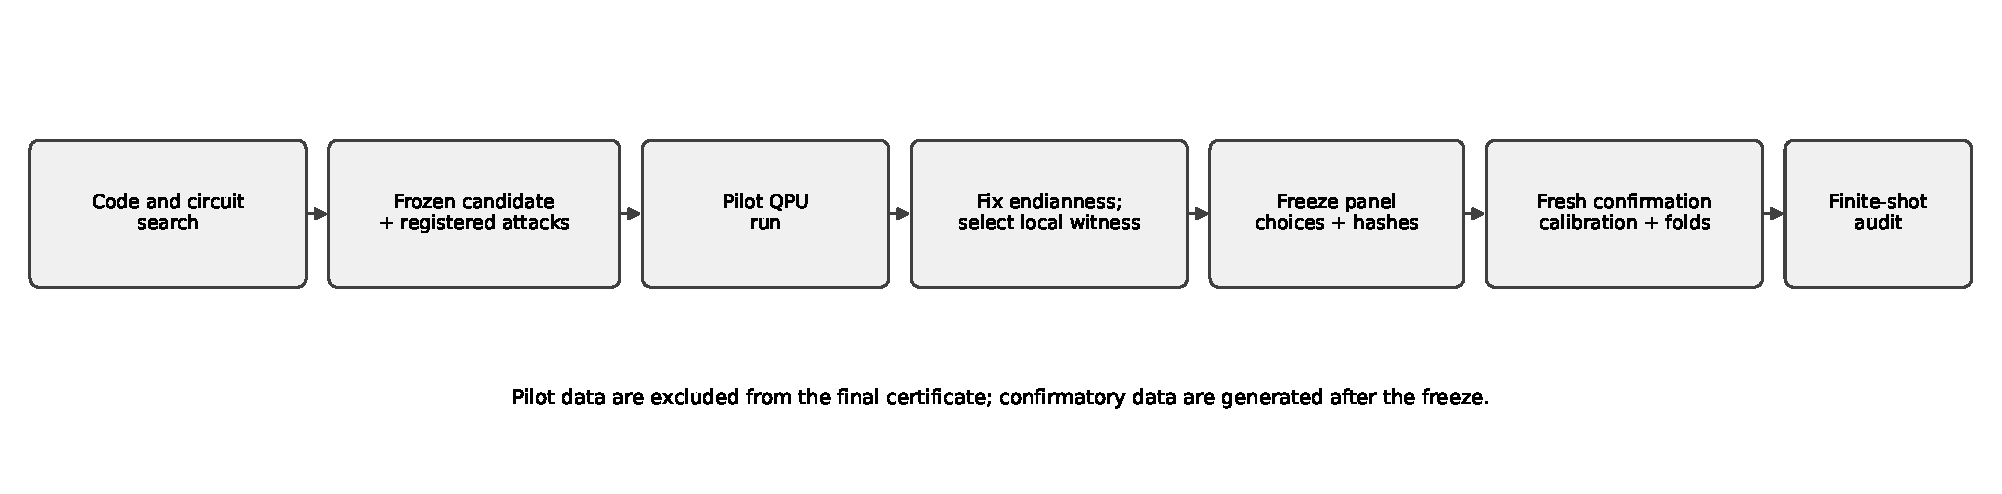
\includegraphics[width=0.99\linewidth]{figures/pilot_confirmatory_workflow.pdf}
\caption{Pilot-confirmatory workflow. Pilot data are used only to correct the convention and select the local witness. The witness, folds, shots, thresholds, and authorization hashes are frozen before fresh confirmatory calibration and science data are analyzed.}
\label{fig:workflow}
\end{figure}

\subsection{Confirmatory campaign and data provenance}
The final campaign comprises:
\begin{itemize}
  \item four pre-science calibration patterns with \num{4000} shots each;
  \item three science circuits at folds 1, 3, and 5, each with \num{10000} shots; and
  \item four post-science calibration patterns with \num{4000} shots each.
\end{itemize}
Thus the confirmatory statistical dataset contains \num{62000} shots. Provider compiler canaries were used only to authorize QASM submission and are not part of the statistical certificate.

\medskip
\noindent\textbf{Confirmatory provenance statement.}
The confirmatory dataset consists of three completed QPU executions at folding factors 1, 3, and 5. The final analysis includes only execution records whose frozen QASM identities and authorization hashes match the preregistered confirmatory panel.

No authentication credentials, account identifiers, organization identifiers, or private provider records are included in the public research package.

\section{Finite-Shot Certificate}
\subsection{Assignment model and drift hull}
Only the two witness coordinates require readout calibration. For each coordinate $j$, the independent assignment channel is
\begin{equation}
M_j\!\left(p^{(j)}_{01},p^{(j)}_{10}\right)=
\begin{pmatrix}
1-p^{(j)}_{01} & p^{(j)}_{10}\\
p^{(j)}_{01} & 1-p^{(j)}_{10}
\end{pmatrix}.
\end{equation}
The four patterns 00, 11, 10, and 01 identify bit convention and assignment errors. Exact Clopper--Pearson intervals~\cite{clopper1934intervals} are constructed separately in pre- and post-periods, with total calibration error budget $\alpha_{\mathrm{cal}}=0.003$. The final uncertainty set $\mathcal{C}$ is the componentwise hull of the pre/post intervals.

The Qiskit bit convention scored 0.9564, compared with 0.4990 for left-to-right interpretation. The convention margin is 0.4574 and the worst assignment-channel determinants are 0.8367 and 0.9292, above the registered threshold 0.75.

The point estimates are reported in \cref{tab:calibration}; the largest pre/post change is 0.0065. \Cref{fig:calibration} visualizes the drift.

\begin{table}[t]
\centering
\caption{Assignment-error point estimates for the two witness coordinates.}
\label{tab:calibration}
\begin{tabular}{@{}lrrr@{}}
\toprule
Parameter & pre & post & absolute drift \\
\midrule
$p^{(39)}_{01}$ & 0.03825 & 0.03175 & 0.00650 \\
$p^{(39)}_{10}$ & 0.09000 & 0.09550 & 0.00550 \\
$p^{(40)}_{01}$ & 0.00875 & 0.01050 & 0.00175 \\
$p^{(40)}_{10}$ & 0.04100 & 0.04075 & 0.00025 \\
\bottomrule
\end{tabular}
\end{table}

\begin{figure}[t]
\centering
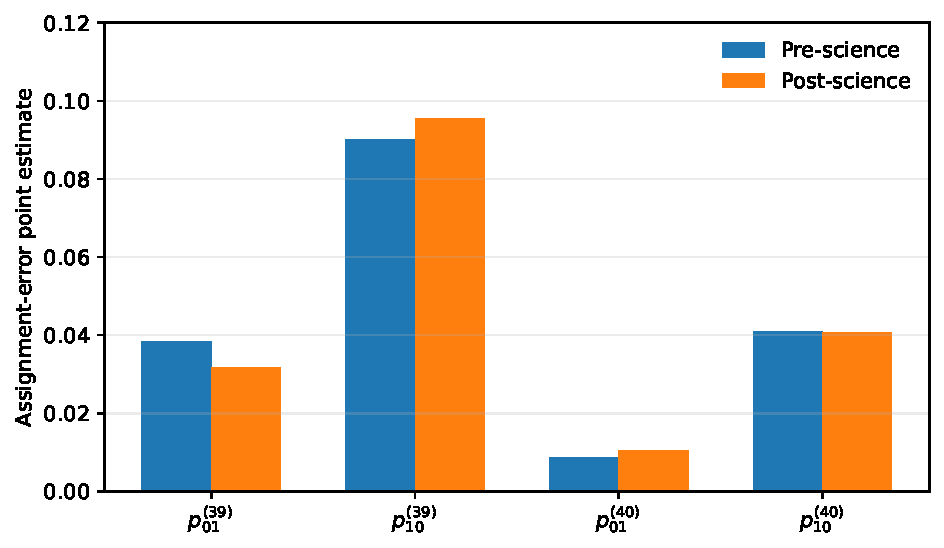
\includegraphics[width=0.82\linewidth]{figures/calibration_drift.pdf}
\caption{Pre- and post-science assignment-error estimates. Confidence intervals, rather than point estimates, define the robust calibration hull used in the certificate.}
\label{fig:calibration}
\end{figure}

\subsection{Readout-corrected local witness}
For a local support $S$, let $M_S=\bigotimes_{j\in S}M_j$ and let $p_S$ be the parity vector with entries $(-1)^{|z|}$. The unbiased inverse-channel coefficient vector is
\begin{equation}
 c_S(\theta)=\left(M_S(\theta)^T\right)^{-1}p_S,
\end{equation}
provided each assignment determinant remains above the registered threshold. The value assigned to a measured two-bit state is the weighted sum of the feature coefficient vectors in the witness.

For $N$ shots, empirical mean $\widehat{\mu}$, sample variance $\widehat{V}$, maximum absolute corrected value $B$, and science error level $\alpha$, the implemented empirical Bernstein lower bound is
\begin{equation}
L(\theta)=\widehat{\mu}(\theta)
-\sqrt{\frac{2\widehat{V}(\theta)\log(3/\alpha)}{N}}
-\frac{6B(\theta)\log(3/\alpha)}{N},
\end{equation}
following the empirical-Bernstein principle~\cite{maurer2009bernstein}. The science error budget is $\alpha_{\mathrm{sci}}=0.007$, divided equally across the three folds, so $\alpha=0.007/3$ per fold.

The calibration-robust observed lower bound is
\begin{equation}
L_s^\star=\inf_{\theta\in\mathcal{C}}L_s(\theta)-10^{-4}.
\end{equation}
Because $\mathcal{C}$ is four-dimensional, all 16 corners are evaluated and a seeded differential-evolution search is additionally applied over the continuous box. The registered adversarial supremum is $A_{\mathrm{adv}}=0.2$ and the generalization penalty is $\delta_{\mathrm{gen}}=0.02$. The certified margin is
\begin{equation}
 m_s=L_s^\star-A_{\mathrm{adv}}-\delta_{\mathrm{gen}}.
\end{equation}
A fold passes when $m_s>0$. The global confirmatory status requires all registered provenance, freshness, QASM, shot, fold, and gap checks in addition to the statistical pass.

\section{Results}
\subsection{Positive margins at all stress levels}
The confirmatory results are shown in \cref{tab:results}. Each circuit has exactly \num{10000} shots. The smallest certified margin is 0.2857977 at fold three; the base-fold margin is 0.2952589. All folds pass.

The critical fold scale is therefore lower-bounded by the largest tested value, $s_{\mathrm{crit}}\geq5$. This statement is limited to the frozen witness, backend state during the campaign, and tested folding construction.

\begin{table}[t]
\centering
\caption{Confirmatory science results. ``Point LCB'' evaluates the finite-shot bound at the center of the calibration box. ``Robust LCB'' minimizes it over the full pre/post hull and includes the $10^{-4}$ safety subtraction.}
\label{tab:results}
\begin{tabular}{@{}rrrrrl@{}}
\toprule
Fold & mean & point LCB & robust LCB & margin & pass \\
\midrule
1 & 0.573715 & 0.536388 & 0.515259 & 0.295259 & yes \\
3 & 0.563608 & 0.526180 & 0.505798 & 0.285798 & yes \\
5 & 0.593331 & 0.556633 & 0.534783 & 0.314783 & yes \\
\bottomrule
\end{tabular}
\end{table}

\begin{figure}[t]
\centering
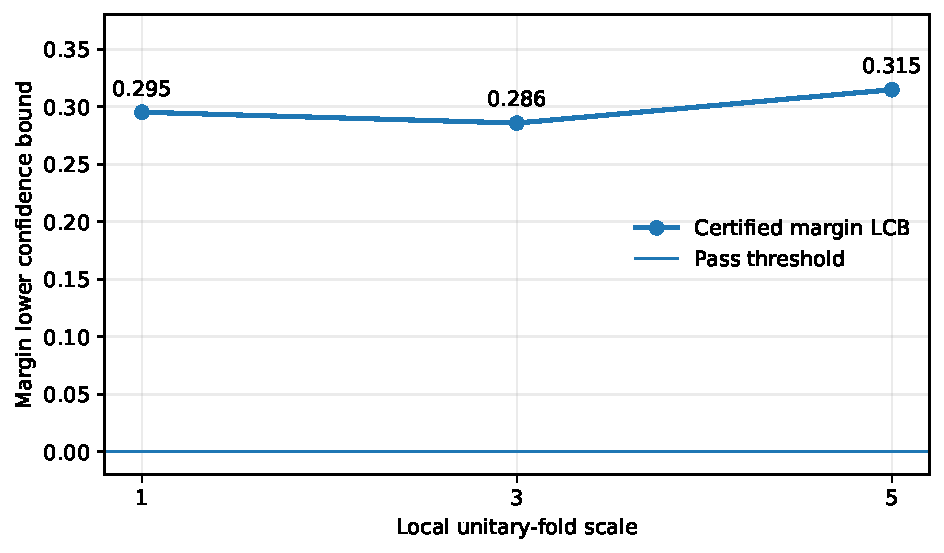
\includegraphics[width=0.82\linewidth]{figures/fold_margins.pdf}
\caption{Certified lower-confidence-bound margin at each local unitary-fold stress level. The registered pass threshold is zero. The nonmonotonic fold response is treated as empirical hardware behavior rather than as a scalar-noise law.}
\label{fig:margins}
\end{figure}

\begin{figure}[t]
\centering
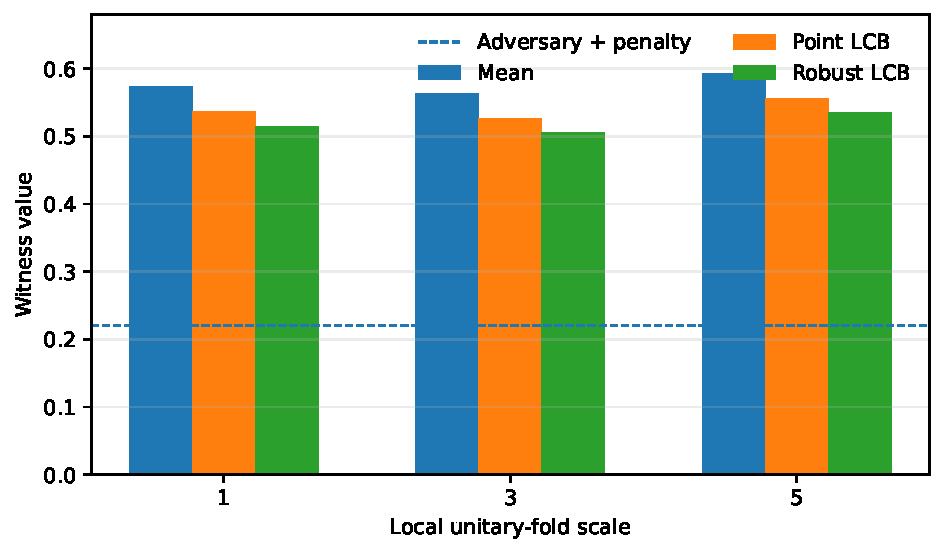
\includegraphics[width=0.82\linewidth]{figures/witness_bounds.pdf}
\caption{Witness mean, point-calibration lower confidence bound, and robust lower confidence bound. The dashed line is the combined adversarial supremum plus generalization penalty, 0.22.}
\label{fig:witness}
\end{figure}

\subsection{Conditional verification/simulation gap}
The registered classical attack suite includes statevector, tensor-network contraction, MPS, Schr\"odinger--Feynman splitting, and stabilizer-decomposition proxies. The best recorded attack is the Cotengra/line-graph contraction estimate~\cite{gray2021hyper}, with $C_{\mathrm{classical}}=\num{96987828}$ operations and contraction width $\log_2\chi=20$. Witness evaluation is assigned $C_{\mathrm{verify}}=27$ operations. The registered gap is
\begin{equation}
 \gamma=\log_{10}\!\left(\frac{C_{\mathrm{classical}}}{C_{\mathrm{verify}}}\right)=6.555353.
\end{equation}
The target $\gamma\geq6$ is met. \Cref{fig:attacks} places the registered proxies on a common logarithmic scale.

\begin{figure}[t]
\centering
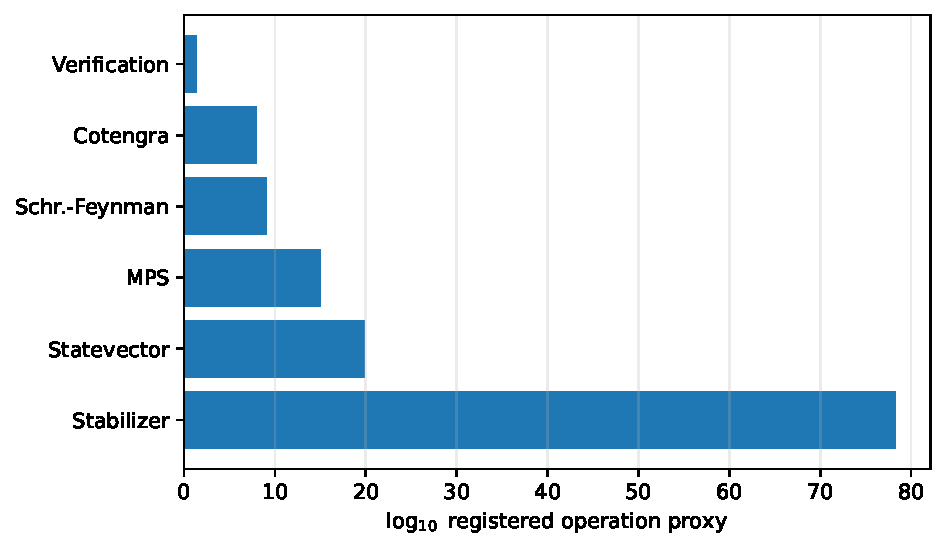
\includegraphics[width=0.82\linewidth]{figures/attack_proxies.pdf}
\caption{Registered operation-count proxies. These are not directly comparable wall-clock measurements and do not exclude unregistered structure-specific attacks.}
\label{fig:attacks}
\end{figure}

\subsection{Provenance and freshness audit}
The final status is \texttt{QPU\_PANEL\_PASS}. The audit verifies that:
\begin{itemize}
  \item the full-width circuit contains both noncommuting axes and the corrected light-cone endianness;
  \item pilot counts are excluded from the final certificate;
  \item confirmatory execution identities are disjoint from pilot identities and their recorded execution times follow the witness freeze;
  \item all science QASM hashes, fold factors, shot counts, and scientific thresholds are unchanged;
  \item provider submission hashes were authorized and QASM semantics were unchanged;
  \item the pre-calibration, three fold-resolved science records, and post-calibration records match the frozen confirmatory panel; and
  \item the final status artifact re-verifies the input freeze manifests before loading the statistical data.
\end{itemize}

\section{Discussion}
The experiment establishes that a local, code-derived witness can retain a positive simultaneous finite-shot margin on a full-width 60-qubit superconducting circuit, even after substantially increasing two-qubit exposure through folds three and five. The calibration drift is small compared with the width of the certified margin, and the result remains positive under worst-case optimization over the pre/post assignment hull.

The most important methodological feature is the separation of design and confirmation. The endianness defect was discovered before the final campaign; the corrected witness was then selected using explicitly declared pilot data, frozen, and tested on disjoint confirmatory executions. This avoids presenting an adaptively selected observable as confirmatory evidence.

The nonmonotonic margin---fold five exceeds fold one---should not be interpreted as noise improving monotonically with circuit depth. Local unitary folding changes duration, coherent-error interference, scheduling, and compilation context. Here folding is a stress test, not a calibrated one-parameter noise model.

The operation-count gap is useful as a red-team target rather than as a final complexity separation. The history of peaked-circuit benchmarks demonstrates that a newly discovered structure-specific classical algorithm can invalidate a broad proxy estimate~\cite{kremer2026peaked}. Accordingly, the frozen $\gamma$ should be updated when stronger attacks are registered, and the public artifacts are intended to make that process straightforward.

The positive result should also be interpreted at the level of the measured observable. A two-feature local parity witness can remain stable even when global distributional features are degraded. This is useful for hardware-oriented protocol design, because it identifies a verifiable signal that is compatible with present calibration and sampling budgets. It is not, by itself, evidence that the entire 60-bit distribution retains the structure required by exact HCS.

\section{Limitations and Non-Claims}
The following boundaries are part of the result:
\begin{enumerate}
  \item \textbf{Not exact HCS.} The experiment does not run the complete HCS logical/syndrome verification procedure and therefore is not an experimental implementation of the exact protocol in Deshpande et al.~\cite{deshpande2025hcs}.
  \item \textbf{No full-distribution certificate.} A positive local witness does not imply closeness in total variation distance to the ideal 60-bit output distribution.
  \item \textbf{Conditional classical gap.} The value $\gamma=6.555$ is relative to a fixed registered attack suite and operation proxies. It is not a proof that no faster classical algorithm exists.
  \item \textbf{No wall-clock advantage.} Verification and simulation operation counts are not a measured quantum-versus-classical runtime comparison.
  \item \textbf{Restricted code optimality.} The trivariate-bicycle instance is the winner only within the frozen search panel and ranking rule.
  \item \textbf{Backend-local robustness.} The fold and calibration conclusions apply to this campaign, backend state, mapping, and witness.
  \item \textbf{Low-weight distance certificate only.} The implementation certifies $d_X,d_Z\geq3$ but does not determine the exact distances.
\end{enumerate}

\section{Outlook}
A direct continuation is to retain the hardware co-design and confirmatory discipline while moving the measured object closer to exact HCS. This requires an explicit logical/syndrome decoder on hardware data, implementation of both peak and syndrome tests, and attacks targeting the joint distribution rather than a two-feature local witness. Other high-value extensions are replication on multiple calibration days, additional independently frozen code instances, cross-backend execution, and public challenge periods for structure-specific classical simulation.

A second direction is to study witness families rather than a single frozen observable. The relevant design problem is to find local or mesoscopic observables whose ideal signal, readout-conditioning, light-cone contraction cost, and adversarial susceptibility remain favorable simultaneously. Such a study should preserve the same pilot/confirmation separation used here.

\section{Data and Code Availability}
The anonymized measurement histograms, frozen circuit descriptions, verification manifests, sanitized QASM files, and analysis metadata supporting the reported certificate are provided as supplementary research artifacts or in a separate archival record. Authentication credentials, account metadata, organization identifiers, provider job identifiers, and private provider records are excluded. The original frozen audit chain is retained privately without alteration.

The public source package contains QASM files named \path{confirmatory-fold-1}, \path{confirmatory-fold-3}, and \path{confirmatory-fold-5}, together with aggregate fold metrics, a machine-readable certificate summary, and publication-compliance documentation. Any later GitHub or Zenodo release should preserve the Open Quantum and Quantum Rings attribution contained in this manuscript and in the accompanying citation metadata.

\section*{Acknowledgments}
Quantum hardware access was provided through Open Quantum, operated by Quantum Rings. This acknowledgment does not imply endorsement by Quantum Rings of the findings, interpretations, or conclusions reported in this work. We separately acknowledge Rigetti Computing as the provider of the Cepheus-1-108Q superconducting quantum processor. Open Quantum and the associated infrastructure are cited according to the platform's research-attribution guidance~\cite{openquantum,openquantumwebsite2026}.

\section{Conclusion}
We demonstrated a positive, independently confirmed local-witness certificate for a 60-qubit code-derived peaked-sampling circuit on a superconducting processor. The certificate survives three unitary-fold stress levels, fresh pre/post calibration uncertainty, and a simultaneous finite-shot analysis. Its scientific value lies as much in the protocol discipline---pilot declaration, frozen choices, disjoint confirmation, immutable hashes, and explicit non-claims---as in the positive margins themselves. The result is a hardware-oriented step toward verifiable code-based sampling experiments, while remaining distinct from an end-to-end implementation of Hidden Code Sampling.

\appendix
\section{Registered Numerical Values}
\begin{table}[H]
\centering
\caption{Frozen values used by the final certificate.}
\begin{tabular}{@{}ll@{}}
\toprule
Quantity & Frozen value \\
\midrule
Backend & \texttt{rigetti:cepheus-1-108q} \\
Candidate identifier & \texttt{654c3ddfe6fe23f2} \\
Code parameters & $n=60$, $k=4$, $\operatorname{rank}H_X=\operatorname{rank}H_Z=28$ \\
Distance statement & $d_X,d_Z\geq3$ under weight-one/two enumeration \\
Witness supports & $\{39,40\}$ and $\{40\}$ \\
Witness weights & $0.8$ and $0.2$ \\
Adversarial supremum & $0.2$ \\
Generalization penalty & $0.02$ \\
Science shots & \num{10000} per fold \\
Calibration shots & \num{4000} per pattern and period \\
Significance allocation & $\alpha_{\mathrm{cal}}=0.003$, $\alpha_{\mathrm{sci}}=0.007$ \\
Optimization safety subtraction & $10^{-4}$ \\
Fold scales & $1,3,5$ \\
Base-fold margin LCB & $0.2952588808$ \\
Minimum margin LCB & $0.2857977493$ \\
Maximum calibration drift & $0.0065$ \\
Registered gap & $\gamma=6.5553534694$ \\
Gap target & $6.0$ \\
Final status & \texttt{QPU\_PANEL\_PASS} \\
\bottomrule
\end{tabular}
\end{table}

\section{Artifact Integrity}
Each private artifact directory contains a \texttt{freeze\_manifest.json} listing relative paths, byte counts, and SHA-256 digests. The final analysis re-verifies all input freezes before loading counts. It also checks raw-count hashes, pilot/confirmation identity disjointness, submission timestamps relative to the panel freeze, provider-QASM authorization, fixed fold factors, fixed shot counts, the corrected endianness convention, and the registered scientific thresholds. The final status itself is frozen after generation.

The public package is a sanitized publication layer rather than a replacement for the immutable private audit chain. Public QASM copies retain the scientific circuit content while omitting account-specific metadata and provider identifiers. Aggregate numerical results can therefore be inspected without exposing authentication material or private provider records.

\section{Open Quantum Publication Compliance}
The public package follows the attribution clause applicable to research outputs derived from Open Quantum Public Compute~\cite{quantumringsterms2026}. In particular:
\begin{itemize}
  \item Open Quantum and Quantum Rings are clearly attributed in the manuscript and public-package metadata;
  \item the official Open Quantum white paper and website are cited;
  \item Rigetti Computing is attributed separately as the hardware provider;
  \item a non-endorsement statement is included;
  \item no Open Quantum, Quantum Rings, or Rigetti logo is used;
  \item credentials, secrets, private account metadata, and provider-specific private records are excluded; and
  \item the original private audit chain remains immutable and separate from the sanitized public release.
\end{itemize}
The official citation page stated on 31 July 2026 that a DOI for the white paper was planned but not yet available; the citation should be checked again immediately before submission~\cite{openquantumcitation2026}.

\printbibliography
\end{document}
